%% -----------------------------------------------------------------
%% This file uses UTF-8 encoding
%%
%% For compilation use following command:
%% latexmk -pdf -pvc -bibtex --shell-escape thesis
%%
%% -----------------------------------------------------------------
%%                                     _     _      
%%      _ __  _ __ ___  __ _ _ __ ___ | |__ | | ___ 
%%     | '_ \| '__/ _ \/ _` | '_ ` _ \| '_ \| |/ _ \
%%     | |_) | | |  __/ (_| | | | | | | |_) | |  __/
%%     | .__/|_|  \___|\__,_|_| |_| |_|_.__/|_|\___|
%%     |_|                                          
%%
%% -----------------------------------------------------------------

\documentclass{kithesis}

% Additional packages
\usepackage[english,slovak]{babel}
\usepackage{blindtext}  % lorem ipsum
%\usepackage{minted}

% Variables
%\thesisspec{figures/thesisspec.png} 

\title{Measurement and interaction of quantum circutis}{Meranie a interakcia kvantových obvodov}

\author{Marián Sabat}
\supervisor{prof. Ing. Ján Kollár, CSc.} %veduci prace
%\consultant{Donald E. Knuth} %konzultant
\college{Techincal University of Kosice}{Technicka Univerzita v Kosiciach} %univerzita
\faculty{Faculty of Electrical Engineering and informatics}{Fakulta elektrotechniky a informatiky} %fakulta
\department{Department of Computers and Informatics}{Katedra počítačov a informatiky} %katedra
\departmentacr{DCI}{KPI} % skratka katedry
\thesis{Master thesis}{Diplomová práca} %typ prace
\submissiondate{1}{1}{2020}
\fieldofstudy{9.2.1 Informatika}
\studyprogramme{Informatika}
%\city{Košice} %mesto
\keywords{Quantum comuters and other key words}{Kvantove pocitace a ine klucove slova}

\declaration{Vyhlasujem, ze vsetko som pisal sam ...}

\abstract{
    % english 
	%\blindtext
	ABSTRAKT
}{
    % slovak 
	%\blindtext
	ABSTRAKT
}

\acknowledgment{%Na tomto mieste by som rád poďakoval svojmu vedúcemu práce za jeho čas a odborné vedenie počas riešenia mojej záverečnej práce.

%Rovnako by som sa rád poďakoval svojim rodičom a priateľom za ich podporu a povzbudzovanie počas celého môjho štúdia.
    
%V neposlednom rade by som sa rád poďakoval pánom {\it Donaldovi E. Knuthovi} a {\it Leslie Lamportovi} za typografický systém \LaTeX, s ktorým som strávil množstvo nezabudnuteľných večerov.
}

\addbibresource{chapters/bibliography.bib}

% if you want to work only on selected chapters
%\includeonly{chapters/analyza} %,chapters/synteza}

% Load acronyms
\newacronym{ny}{NY}{New York}
\newacronym{la}{LA}{Los Angeles}
\newacronym{un}{UN}{United Nations}
\newacronym{gcd}{GCD}{Greatest Common Divisor}
\newacronym{lcm}{LCM}{Least Common Multiple}


%% -----------------------------------------------------------------
%%          _                                       _   
%%       __| | ___   ___ _   _ _ __ ___   ___ _ __ | |_ 
%%      / _` |/ _ \ / __| | | | '_ ` _ \ / _ \ '_ \| __|
%%     | (_| | (_) | (__| |_| | | | | | |  __/ | | | |_ 
%%      \__,_|\___/ \___|\__,_|_| |_| |_|\___|_| |_|\__|
%%                                                      
%% -----------------------------------------------------------------

\begin{document}
%% Title page, abstract, declaration etc.:
\frontmatter{}

%% List of code listings, if you are using package minted
%\listoflistings

\pagenumbering{arabic}

%% Chapters
% !TEX root = ../thesis.tex

\chaptermark{Úvod}
\addcontentsline{toc}{chapter}{Úvod}

\chapter*{Úvod}

Systémy, ktoré sa dokážu učiť z dát sú už dnes prístupné verejnosti. Je čoraz jednoduchšie študovať techniky strojového učenia a preto progres v tomto odvetví je skutočne viditeľný. Množstvo dát a dobrá výpočtová technika majú za následok, že v takmer všetkých oblastiach sa zavádza nejaký druh umelej inteligencie. Počítače, ktoré by rozumeli informáciám by znamenali revolúciu v našich životoch. Program, ktorý by dokázal vygenerovať obraz na základe hudobného podkladu, na základe emócií a nálad, ktoré sú obsiahnuté v hudbe by bol pokrok ku umelej inteligencii, ktorá by skutočne rozumela dátam.

Proces syntézy jedného druhu informácií na iní je pre ľudí prirodzený no pre stroj je to neľahká úloha. Avšak progres v neurónových sieťach a v generatívnych algoritmoch umožňuje klasifikáciu jednej informácie a jej následnú zmenu na inú formu. Stále ale existuje množstvo prekážok v realizácií tohto problému.

To všetko nás privádza k otázke, sú dnešné neurónové siete schopné previesť hudobnú skladbu na zmysluplný obraz?
Prevod hudobnej informácie na obrazovú si vyžaduje určitý stupeň kreativity a znalostí. 
V našej práci sa budeme snažiť zodpovedať tento problém.
Budeme sa snažiť vytvoriť model, ktorý by simuloval ľudskú kreativitu.

V prvom rade je dôležité upraviť dáta, ktoré budeme analyzovať. Ide o zvukové signály, ktoré ako také sú nespracovateľné dnešnými algoritmami strojového učenia.
Je nevyhnutné aby sme tieto dáta upravili na použiteľnú formu.
Ďalším krokom je zistenie či sú počítače vôbec schopné priradenia najjednoduchšej obrazovej formy, čiže farby, k hudobným skladbám.
Úspešné splnenie tejto úlohy bude dobrým predpokladom pre vytvorenie finálneho modelu, ktorý dokáže generovať obrázky na vyššej kreatívnej úrovni.

Naša práca je preto rozdelená presne podľa týchto celkov.
Prvé kapitoly poskytnú súčasné úspechy v syntéze dát a teoretický základ pre naše riešenie.
V ďalších kapitolách postupne prejdeme naše výsledky od najjednoduchších modelov až po tie zložitejšie.
Na konci poskytneme porovnanie nami vytvorených systémov a odvodenie záverov.  

% !TEX root = ../thesis.tex

\chapter{Ciele prace (Formulacia ulohy)}

%Text záverečnej práce musí obsahovať\/ kapitolu s~formuláciou úlohy resp. úloh riešených v~rámci záverečnej práce. V~tejto časti autor rozvedie spôsob, akým budú riešené úlohy a~tézy formulované v~zadaní práce. Taktiež uvedie prehľad podmienok riešenia.


% !TEX root = ../thesis.tex

\chapter{Matematické základy kvantových systémov}

Na pochopenie problematiky kvantových počítačov je nutná znalosť aspoň základnej lineárnej algebry.
V tejto kapitole je opísaný matematický aparát využívaný ako teoretický základ celej práce.

\section{Matice}

Maticou typu \(m \times n\) je nazývaná sústava prvkov zapísaných do schémy s \(m\) riadkami a \(n\) stĺpcami, kde \(n,m \in \field{N}\) \cite{Ste18}.
Teda:
\[
A = \begin{bmatrix}
		a_{11} & a_{12} & \dots & a_{1n} \\
		a_{21} & a_{22} & \dots & a_{2n} \\
		{...}							\\
		a_{m1} & a_{m2} & \dots & a_{mn}
     \end{bmatrix}
\]

\subsection{Násobenie matice skalárom}
Toto násobenie je vykonané násobením každého prvku matice danou skalárnou hodnotou \cite{Ste18}.
Majme maticu \(A\) typu \(2 \times 2\) a skalárnu hodnotu \(k\), potom platí
\[
kA = k \begin{bmatrix}
		 a_{11} & a_{12} \\
		 a_{21} & a_{22}
       \end{bmatrix}
= \begin{bmatrix}
	ka_{11} & ka_{12} \\
	ka_{21} & ka_{22}
  \end{bmatrix}
\]
Operácia násobenia matice skalárnou hodnotou je komutatívna, čiže na poradí operandov nezáleží.
Nech \(B\) je matica a \(\alpha, \beta\) sú skalárne hodnoty, potom
\[(\alpha + \beta)B = \alpha B + \beta B,\] \[(\alpha \beta)B = \alpha(\beta B)\]

\subsection{Násobenie matíc}
Nech je daná matica \(A\) typu \(m \times n\) a matica \(B\) typu \(n \times p\), potom výsledná matica \(C = AB\) je typu \(m \times p\) a pre jej prvky platí
\[c_{ij} = \sum_{k=1}^{n} A_{ik}B_{kj} = A_{i1}B_{ij} + \dots + A_{in}B_{nj},\]
kde \(i = 1, \dots ,m\), a \(j = 1, \dots , p\) \cite{Ste18}.
Pre túto operáciu neplatí komutatívnosť.

\subsection{Transpozícia matice}
Ak \(A\) je matica typu \(m \times n\), potom jej transponovaná matica \(A^{T}\) je typu \(n \times m\) a platí \cite{Ste18} \[(A^{T})_{ij} = A_{ji}\]

\subsection{Tenzorový súčin matíc}
Nech \(A\) je matica typu \(m \times n\) a \(B\) je typu \(r \times s\).
Tenzorový súčin alebo Kroneckerov súčin, označený ako \(A \otimes B\) je definovaný ako \cite{Gra81}
 \[
A \otimes B = \begin{bmatrix}
		a_{11}B & a_{12}B & \dots & a_{1n}B \\
		a_{21}B & a_{22}B & \dots & a_{2n}B \\
		{...}							\\
		a_{m1}B & a_{m2}B & \dots & a_{mn}B
     \end{bmatrix}
\]
Nakoľko je \(a_{ij}B\) submatica typu \(r \times s\), je zjavné, že výsledná matica je typu \(mr \times ns\).

\section{Komplexné čísla}
Množinou komplexných čísel \(\field{C}\) je nazývaná množina \(\field{R}^2\) spolu s operáciami sčítania a násobenia. Ľubovoľný prvok \(z = (a, b) \in \field{C}\) je nazývaný komplexné číslo \cite{Tit06}.
Komplexné čísla možno reprezentovať nie len ako usporiadanú dvojicu, ale aj pomocou:
\begin{enumerate}
\item Algebraickej formy \[z = a + bi\], kde \(a,b \in \field{R}\) a \(i^{2} = -1\),
\item Polárnych súradníc \(\rho\) a \(\varphi\), \\
kde \(\rho,\varphi \in \field{R}\) a \(\rho > 0\).
V geometrickej reprezentácii (Obr. \ref{fig:kn}) je \(\rho\) veľkosť vektora \(\vec{Oz}\), kde \(O\) je počiatok súradnicovej sústavy, a \(\varphi\) je uhol medzi osou \(x\) a daným vektorom.
\end{enumerate}
Je zrejme, že pre vyjadrenie pomocou polárnych súradníc platí \(a = \rho \cos \varphi\) a \(b = \rho \sin \varphi\) \cite{Tit06}.
Potom je možné zapísať \[z = \rho e^{i \varphi}\] ,kde \(z \in \field{C}\), \(\rho , \varphi \in \field{R}\) a \(\rho > 1\).
\(e^{i \varphi}\) je komplexná jednotka, inak povedané jej absolútna hodnota je rová 1.
\[|e^{i \varphi}| = 1\]
A z Eulerovho vzťahu platí
\[e^{i \varphi} = \cos \varphi + i\sin \varphi\]

\begin{figure}
\centering
\begin{tikzpicture}[scale=2]
\coordinate (O) at (0,0);
\coordinate (A) at ($({1/sqrt(2)},0)$);
\coordinate (B) at ($({1/sqrt(2)},{1/sqrt(2)})$);

\draw [-latex] (-2,0) -- (2,0) node[below left]{x};
\draw [-latex] (-2,0) -- (2,0) node[above left]{Re$\,z$};
\draw [-latex] (0,-1.5) -- (0,1.5) node[below right]{y};
\draw [-latex] (0,-1.5) -- (0,1.5) node[below left]{Im$\,z$};
\draw (O)--(A)--(B)--cycle;
\draw (O) circle(1);

\tkzLabelSegment[below](O,A){\(a\)}
\tkzLabelSegment[left](A,B){\(b\)}
\tkzLabelSegment[above](O,B){\(\rho\)}

\tkzMarkAngle[size=.4](A,O,B)
\tkzLabelAngle[pos=.3](A,O,B){\(\varphi\)}

\end{tikzpicture}
\caption{Zobrazenie komplexného čísla z: x - reálna os, y - imagináran os}
\label{fig:kn}
\end{figure}

\subsection{Operácie na množine komplexných čísel}
\textbf{Súčet komplexných čísel}
\begin{itemize}
\item \((a + bi) + (c + di) = (a + c) + (b + d)i\)
\item \(\rho_{1}e^{i \varphi_{1}} + \rho_{2}e^{i \varphi_{2}} = \rho_{1}(\cos \varphi_{1} + i\sin \varphi_{1}) + \rho_{2}(\cos \varphi_{2} + i\sin \varphi_{2}) =  (\rho_{1}\cos \varphi_{1} + \rho_{2}\cos \varphi_{2}) + i(\rho_{1}\sin \varphi_{1} + \rho_{2}\sin \varphi_{2})\)
\end{itemize}

\textbf{Násobenie komplexných čísel}
\begin{itemize}
\item \((a + bi)(c + di) = ac + adi + bci - bd = (ac - bd) + (ad + bd)i\)
\item \(\rho_{1}e^{i \varphi_{1}} . \rho_{2}e^{i \varphi_{2}} = \rho_{1} \rho_{2}e^{i(\varphi_{1} \varphi_{2})}\)
\end{itemize}

Operácie rozdielu a podielu sú ľahko odvoditeľné obnobným spôsobom.

\subsection{Základné charakteristiky komplexných čísel}
Nech \(\alpha\) je komplexné číslo \(\alpha = a + bi, \alpha \in \field{C}\).
Potom hovoríme, že \(a,b\) sú zložky komplexného čísla \(\alpha\), pričom \(a\) je reálna a \(b\) je imaginárna zložka.
Pri reprezentácii pomocou polárnych súradníc \(\alpha = \rho e^{i\varphi}\) je \(\rho\) nazývané amplitúda (veľkosť, norma) komplexného čísla a \(\varphi\) je fáza komplexného čísla. \\

Pre komplexné číslo \(\alpha \in \field{C}\) je číslo \(\alpha^{\dag}\) (\(\overline{\alpha}\) alebo \(\alpha^{*}\)) nazývané združeným komplexným číslom (angl. conjugate of complex number) \cite{Tit06}, pričom ak \(\alpha = a + bi\), potom 
\[\alpha^{\dag} = a - bi,\] 
\[\alpha^{\dag} = \rho e^{-i\varphi}.\]
Z geometrickej reprezentácie komplexného čísla na Obr. \ref{fig:kn} je zrejmé, že \(\rho = \sqrt{a^2 + b^2}\).
Bolo už spomenuté, že \(\rho\) sa nazýva aj norma komplexného čísla.
Normu komplexného čísla \(\alpha\) možno označiť aj ako \(|\alpha|\) a platí
\[|\alpha| = \sqrt{\alpha^{\dag}\alpha}.\]
Dôkaz:
\[|\alpha| = \sqrt{\alpha^{\dag}\alpha} = \sqrt{\rho e^{-i\varphi}.\rho e^{i\varphi}} = \sqrt{\rho^{2}} = \rho\]

\section{Vektory}
\label{vektory}

Vektor rozmeru \(n\) je usporiadaný súbor prvkov.
Vo všeobecnosti je možné vektor \(A\) označiť ako 
\[A = \begin{pmatrix}
		a_{1} \\
		a_{2}\\
		\dots \\
		a_{n}
     \end{pmatrix}\]
No je žiadúce označovať vektory pomocou Diracovho (Bra-ket) zápisu.
Čiže vektory \(u = \binom{\alpha}{\beta}\) a \(v = \binom{\gamma}{\delta}\) je lepšie označiť ako 
\[\Ket{\psi_1} = \binom{\alpha_1}{\beta_1}\]
\[\Ket{\psi_2} = \binom{\alpha_2}{\beta_2}\]
Toto označenie popisuje vektory v Hilbertovom priestore (viac v kapitole \ref{hil_space}), pričom platí nasledovné:

Ak \(\Ket{\psi} = \binom{\alpha}{\beta}\) je ket-vektor, potom 
\[\Bra{\psi} = {\binom{\alpha}{\beta}}^{\dag} = (\alpha^{\dag} \beta^{\dag})\]
je  bra-vektor, kde \( ( \alpha, \beta, \alpha^{\dag}, \beta^{\dag} \in \field{C} ) \) a \(\alpha^{\dag}, \beta^{\dag}\) sú združené komplexné čísla ku \(\alpha\) a \(\beta\).
\(\Bra{\psi}\) je teda združenou transpozíciou (angl. transposed conjugate), a platí
\[\Bra{\psi^{\dag}} = \Ket{\psi}\]
\[\Ket{\psi^{\dag}} = \Bra{\psi}\]


\section{Pojmi a definície}
Vektor je \textbf{normalizovaný}, ak jeho norma (veľkosť) je rovná 1.
\[\left\Vert \binom{\alpha}{\beta} \right\Vert = \sqrt{|\alpha|^2 + |\beta|^2}= 1\]

Vektory \(\psi_1\) a \(\psi_2\) sú navzájom \textbf{ortogonálne}, ak ich skalárny súčin je rovný 0. Ortogonálnosť (angl. orthogonality) je v tomto ponímaní teda možné zameniť s kolmosťou.

Dva vektory sú \textbf{ortonormálne}, ak sú zároveň ortogonálne a normalizované.

Pre príklad nech \(\Ket{0} = \binom{1}{0}\) a \(\Ket{1} = \binom{0}{1}\), \( (\Ket{0}, \Ket{1} \in \field{C}^2) \).
Tieto vektory sú ortonormálne, pretože platí 
\begin{enumerate}
\item \(\Braket{0|1} = \Bra{0} . \Ket{1} = \Ket{0^{\dag}} . \Ket{1} = (1 0) . \binom{0}{1} = 0,\)
\item \(\Vert \Ket{0} \Vert^2 = \Braket{0|0} = (1 0) . \binom{1}{0} = 1\) \\
\(\Vert \Ket{1} \Vert^2 = \Braket{1|1} = (0 1) . \binom{0}{1} = 1\).
\end{enumerate}

Pre \textbf{skalárny súčin} dvoch vektorov platí
\[\Braket{\psi_1|\psi_2} = \Bra{\psi_1} . \Ket{\psi_2} = (\alpha_1^{\dag}\beta_1^{\dag}) . \binom{\alpha_2}{\beta_2} = \alpha_1^{\dag}\alpha_2 + \beta_1^{\dag}\beta_2.\]

\textbf{Normu} vektora \(\Ket{\psi}\) pomocou skalárneho súčinu je možné vypočítať ako
\[\Vert \Ket{\psi} \Vert = \sqrt{\Braket{\psi|\psi}},\]
pretože platí \(\Braket{\psi|\psi} = \alpha^{\dag}\alpha + \beta^{\dag}\beta = |\alpha|^2 + |\beta|^2 = \Vert \Ket{\psi} \Vert^2\).

Operácia \textbf{tenzorového súčinu} dvoch vektorov je definovaná ako
\[
\Ket{\psi_1} \otimes \Ket{\psi_2} = \Ket{\psi_1} . \Bra{\psi_2} = \binom{\alpha_1}{\beta_1} . (\alpha_2\beta_2) = 
\begin{pmatrix}
	\alpha_1(\alpha_2\beta_2) \\ 
	\beta_1(\alpha_2\beta_2)
\end{pmatrix} = 
\begin{pmatrix}
	\alpha_1\alpha_2 \quad \alpha_1\beta_2 \\
	\beta_1\alpha_2 \quad \beta_1\beta_2
\end{pmatrix}
\]

% !TEX root = ../thesis.tex

\chapter{Teoretické základy kvantových systémov}

V nasledujúcej kapitole sú uvedené poznatky z teórie kvantových výpočtov a kvantových obvodov.

\section{Základné definície}

\begin{itemize}
\item[] \textbf{Hilbertov priestor} \\
\label{hil_space}
Hilbertov priestor (angl. Hilber space) je úplný konečnorozmerný vektorový priestor, v ktorom je definovaná operácia skalárneho súčinu \(\Braket{u|v}\), kde \(u,v\) sú \(N\)-rozmerné vektory s komplexnými zložkami \cite{Nie10}.
Konečnorozmerným vektorovým priestorom nazývame taký priestor, ktorého báza je množina lineárne nezávislých  vektorov, a ktorá generuje celý tento priestor.
Pre úplný priestor platí, že existuje Cauchyho postupnosť, ktorou je dosiahnuteľný ľubovoľný stav, charakterizovateľný \(N\)-rozmerným vektorom \(\Ket{\psi} \in \field{C}^{N}\), ktorý je vždy normalizovaý.

\item[] \textbf{Unitárne zobrazenie} \\
Unitárne zobrazenie (angl. Unitary map) je rotáciou, čiže zmenou ortonormálnej bázy.

\item[] \textbf{Kvantový bit} \\
Za kvantový bit je možné považovať objekt, ktorý popisuje stav kvantového systému.
Z matematického pohľadu je to vektor v dvojrozmernom Hilberovom priesotre \(\field{C}^{2}\).
No v reále ide o fotón.
Budeme sa zaoberať dvojstavovými kvantovými systémami, kde je fotón nútený skolabovať do jedného z dvoch stavov.
A teda vektor, ktorý bude popisovať tento kvantový bit vyjadríme ako \(u = \binom{\alpha}{\beta}\), \( ( \alpha, \beta \in \field{C} ) \) a \(u \in \field{C}^{2}\) \cite{Kay07}.
No vhodnejším sa javí vyjadrenie tohto vektora superpozíciou, teda lineárnou kombináciou základných stavov \(\Ket{0}, \Ket{1}\), ktoré zodpovedajé klasickým bitom \(0,1\).
Teda \[u = \binom{\alpha}{\beta} = \alpha \binom{1}{0} + \beta \binom{0}{1} = \alpha\Ket{0} + \beta\Ket{1},\]
kde monožina \(\{\Ket{0}, \Ket{1}\} = \{\binom{1}{0}, \binom{0}{1}\}\) je nazývaná základná báza.
Väčšinou je využívaná základná báza \(\{\Ket{0}, \Ket{1}\}\), no je možné sa stretnúť aj s bázami \(\{\Ket{+}, \Ket{-}\}\) a \(\{\Ket{\circlearrowright}, \Ket{\circlearrowleft}\}\). Tieto bázy sú dosiahnuteľné zo základnej bázy unitárnymi transformáciami.

\item[] \textbf{Superpozícia} \\
Superpozíciou (angl. superposition) dvoch vektorov je vyjadrený stav kvantového bitu \(\Ket{\psi}\), \(\Ket{\psi} \in \field{C}^2\).
Ide o lineárnu kombináciu a teda vo všeobecnosti tieto vektory môžu byť dva ľubovoľné, no lineárne nezávislé vektory \(u\) a \(v\). Čiže
\[\Ket{\psi} = \alpha u + \beta v.\]
Pre kvantové výpočty, ale má väčší význam využitie ortonormálnych vektorov.
\[\Ket{\psi} = \alpha \Ket{0} + \beta \Ket{1},\]
\[\Ket{\psi} = \alpha \Ket{+} + \beta \Ket{-},\]
\[\Ket{\psi} = \alpha \Ket{\circlearrowright} + \beta \Ket{\circlearrowleft},\]
kde \(\alpha, \beta \in \field{C}\) a platí \(|\alpha|^2 + |\beta|^2 = 1\).

\item[] \textbf{Previazanosť kvantových bitov} \\
(Quantum Computation and Quantum Information) Majme stav dvoch qbitov
\[\Ket{\psi} = \frac{\Ket{00} + \Ket{11}}{\sqrt{2}}\]
Pre tento stav neexistuje taká dvojica stavov \(\Ket{a}\) a \(\Ket{b}\), že platí \(\Ket{\psi} = \Ket{a}\Ket{b}\).
Hovoríme, že stav zloženého systému, ktorý nemožno zapísať ako súčin stavov jeho komponentov sa nazýva previazaným (angl. entagled) stavom.

V prípade jednoduchého n-bitového kvantového systému môžme jeho celkový stav \(\Ket{\psi}\) vyjadriť tenzorovým súčinom vektorov stavov jednotlivých bitov \(\Ket{\psi_0}\), \(\Ket{\psi_1}\), \(\dots\), \(\Ket{\psi_{n-1}}\).
Čiže
\[\Ket{\psi} = \Ket{\psi_0} \otimes \Ket{\psi_1} \otimes \dots \otimes \Ket{\psi_{n-1}}\]
Toto však neplatí, ak dva alebo viac kvantových bitov je navzájom previazaných.
Pretože previazané bity sú charakteristické rovnakými vektormi, a to počas celého výpočtu a aj pri meraní.
\end{itemize}

\section{Systém s jedným kvantovým bitom}
\[\Ket{\psi} = \binom{\alpha}{\beta} = \binom{\alpha}{0} + \binom{0}{\beta} = \alpha \binom{1}{0} + \beta \binom{0}{1} = \alpha \Ket{0} + \beta \Ket{1}, \]
kde \(\alpha, \beta \in \field{C}\) a \(\Ket{\psi} \in \field{C}^{2}\).
Čiže stav kvantového systému \(\Ket{\psi}\) je superpozíciou stavov \(\Ket{0}\) a \(\Ket{1}\).
\[\Ket{\psi} = \binom{\alpha}{\beta}\]
\[\Bra{\psi} = (\alpha^{\dag}\beta^{\dag})\]
\[\Braket{\psi|\psi} = (\alpha^{\dag}\beta^{\dag})\binom{\alpha}{\beta} = \alpha^{\dag}\alpha + \beta^{\dag}\beta = |\alpha|^{2} + |\beta|^{2} = ||\Ket{\psi}||^{2}\]


\section{System s viacerymi kvantovymi bitmy}
\section{Princip merania}

% !TEX root = ../thesis.tex

\chapter{Kvantový systém}

Stupeň vývoja kvantových počítačov nateraz neumožňuje priamy prístup k
fyzickému stroju. Tieto prototypy sú veľmi veľké a prísne strážené v 
laboratóriách. Našťastie existujú nástroje, ktorými je umožnená práca aj 
obyčajným ľuďom. Jedným z najpoužívanejším nástrojom je IBM Quantum Experience
\cite{IBM}. 

\section{IBM Quantum Experience}
IBM Quantum Experience (ďalej len IBM QX) je webová aplikácia, ktorá 
slúži na experimentovanie s kvantovým počítačom. Medzi jej funkcionality 
možno zahrnúť vytváranie a ukladanie kvantových obvodov, ako aj ich 
vykonávanie na kvantovom počítači. Tento počítač je simulovaný virtuálny 
stroj, no IBM QX umožňuje aj odoslanie experimentu na reálny počítač. 
Simulátor umožňuje relatívne rýchlu prácu s kvantovým počítačom. Tento
prístup odľahčuje skutočný systém od veľkej sieťovej premávky a takisto 
zlepšuje používateľský zážitok.

Vytáranie nového obvodu je veľmi intuitívne. Na obrázku \ref{ibm_qx_composer}
je nástroj na to určený. Prednastavené hradlá je spôsobom ťahaj a pusť (angl.
drag and drop) možné presúvať na plán kvantového obvodu. Po uložení je možné
naštartovať tento program. Na server sa odošle experiment, za predpokladu, že
je obvod vykonávaný na simulátore, tak za krátku dobu dostaneme vrátené 
výsledky.

\begin{figure} 
	\centering 
	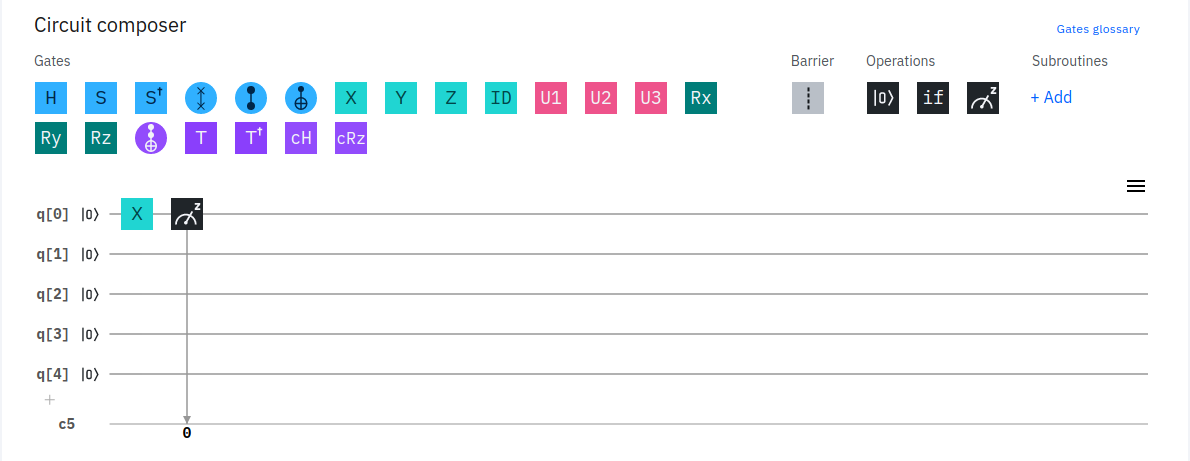
\includegraphics[width=1\textwidth]{figures/ibm_qx_composer.png} 
	\caption{Nástroj na tvorbu kvantových obvodov v IBM Quatnum Experience.}
    \label{ibm_qx_composer}
\end{figure}

Obvody je možné navrhovať aj pomocou špeciálneho jazyka OpenQASM, pomocou
editora, ktorý IBM QX obsahuje. Pri zobrazovaní výsledkov sa stav systému 
označuje pomocou klasických bitov. Teda pri navrhovaní programu pomocou
OpenQASM, je nutné definovať jednak počet kvantových a súčasne aj počet 
klasických bitov v systéme.

\begin{code}
qreg q[5];
creg c[5];
\end{code}

Je dôležité podotknúť, že kvantový bit \(\psi_0\) je v IBM QX reprezentovaný
ako \(q[0]\), \(psi_1 = q[1]\) a tak ďalej. Pri meraní sa tieto bity zobrazia
do príslušných c registrov:
\begin{itemize}
\item[] \(q[0] \rightarrow c[0]\)
\item[] \(q[1] \rightarrow c[1]\)
\item[] \(\dots\)
\end{itemize}

Po inicializácií potrebných registrov je možné pristúpiť k definovaniu 
samotného obvodu. Pre dosiahnutie obvodu ako na obrázku \ref{ibm_qx_composer}
vyvoláme aplikáciu hradla \(X\) na bite \(q[0]\) a následne využijeme meranie.

\begin{code}
x q[5];
measure q[0] -> c[0];
\end{code}

\begin{figure} 
	\centering 
	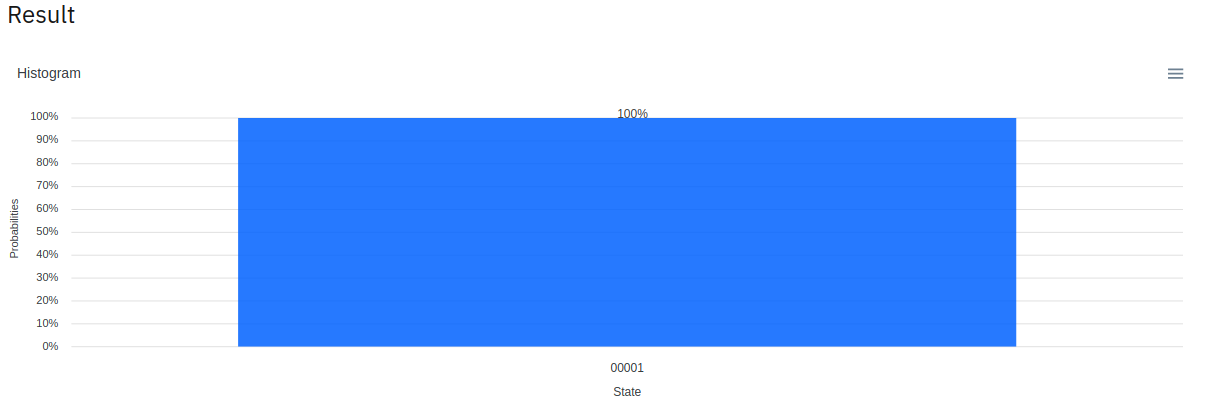
\includegraphics[width=1\textwidth]{figures/ibm_qx_results.png} 
	\caption{Výsledky experimentu z IBM Quantum Experience.}
    \label{ibm_qx_results}
\end{figure}

Výsledky experimentov sa zobrazujú v stĺpcovom diagrame, pričom stav systému
je zobrazovaný v klasických bitoch opačne ako v kvantových. Teda stav 
n-bitového systému \(\psi = \Ket{\psi_0\psi_1\psi_2 \dots \psi_{n-1}}\) je
meraný do klasického registra ako 
\[c_{n-1} \dots c_2 c_1 c_0\]
V našom prípade je
\[q[0] = X \Ket{0} =
\begin{pmatrix}
0 & 1\\
1 & 0\\
\end{pmatrix}
\binom{1}{0} = \binom{0}{1}
,\]
čo je \(1\) s pravdepodobnosťou \(1\). Výsledok na obrázku 
\ref{ibm_qx_results} zobrazuje, že kvantový systém dosiahne so \(100\%\) 
pravdepodobnosťou stav \(00001\).

\subsection{Stavy a ich zápis}

Pri výpočtoch je najviac využívaných týchto šesť stavov kvantových bitov 
\cite{Wei02}:
\begin{enumerate}
\item \(\Ket{0} = \binom{1}{0}\),
\item \(\Ket{1} = \binom{0}{1}\),
\item \(\Ket{+} = \frac{\Ket{0} + \Ket{1}}{\sqrt{2}}\),
\item \(\Ket{-} = \frac{\Ket{0} - \Ket{1}}{\sqrt{2}}\),
\item \(\Ket{\circlearrowright} = \frac{\Ket{0} - i\Ket{1}}{\sqrt{2}}\),
\item \(\Ket{\circlearrowleft} = \frac{\Ket{0} - i\Ket{1}}{\sqrt{2}}\).
\end{enumerate}
Zmena stavu kvantového bitu je možná pomocou hradiel. Existuje viacero
hradiel, ktoré možno používať v kvantových systémoch. Aplikovaním hradiel
na rôznych stavoch dosiahneme rôznu zmenu. Prehľad aplikácií základných 
hradiel je v~tabuľke \ref{hradla_vysl}.

\begin{table}
\begin{tabular}{|c|c||c|c|c|c|c|c|}
\hline
 & & \(\Ket{0}\) & \(\Ket{1}\) & \(\Ket{+}\) & \(\Ket{-}\) & \(\Ket{\circlearrowright}\) & \(\Ket{\circlearrowleft}\) \\
\hline
 & & \(\binom{1}{0}\) & \(\binom{0}{1}\) & \(\frac{1}{\sqrt{2}} \binom{1}{1}\) & \(\frac{1}{\sqrt{2}} \binom{1}{-1}\) & \(\frac{1}{\sqrt{2}}\binom{1}{i}\) & \(\frac{1}{\sqrt{2}} \binom{1}{-i}\) \\
\hline

\(X\) &  \(\begin{pmatrix}
0 & 1\\
1 & 0\\
\end{pmatrix} \) & \(\binom{0}{1}\) & \(\binom{1}{0}\) & \(\frac{1}{\sqrt{2}} \binom{1}{1}\) & \(\frac{1}{\sqrt{2}} \binom{-1}{1}\) & \(\frac{1}{\sqrt{2}} \binom{i}{1}\) & \(\frac{1}{\sqrt{2}} \binom{-i}{1}\) \\
\hline

\(Y\)  &  \(\begin{pmatrix}
0 & -i\\
i & 0\\
\end{pmatrix} \) & \(\binom{0}{i}\) & \(\binom{-i}{0}\) & \(\frac{1}{\sqrt{2}} \binom{-i}{i}\) & \(\frac{1}{\sqrt{2}} \binom{i}{i}\) & \(\frac{1}{\sqrt{2}} \binom{1}{i}\) & \(\frac{1}{\sqrt{2}} \binom{-1}{i}\) \\
\hline

\(Z\)  &  \(\begin{pmatrix}
1 & 0\\
0 & -1\\
\end{pmatrix} \) & \(\binom{1}{0}\) & \(\binom{0}{-1}\) & \(\frac{1}{\sqrt{2}} \binom{1}{-1}\) & \(\frac{1}{\sqrt{2}} \binom{1}{1}\) & \(\frac{1}{\sqrt{2}} \binom{1}{-i}\) & \(\frac{1}{\sqrt{2}} \binom{1}{i}\) \\
\hline

\(H\)  &  \(\frac{1}{\sqrt{2}}\begin{pmatrix}
1 & 1\\
1 & -1\\
\end{pmatrix} \) & \(\frac{1}{\sqrt{2}}\binom{1}{1}\) & \(\frac{1}{\sqrt{2}}\binom{1}{-1}\) & \(\binom{1}{0}\) & \(\binom{0}{1}\) & \(\frac{1}{\sqrt{2}} \binom{\frac{1+i}{\sqrt{2}}}{\frac{1-i}{\sqrt{2}}}\) & \(\frac{1}{\sqrt{2}} \binom{\frac{1-i}{\sqrt{2}}}{\frac{1+i}{\sqrt{2}}}\) \\
\hline

\(S\)  &  \(\begin{pmatrix}
1 & 0\\
0 & i\\
\end{pmatrix} \) & \(\binom{1}{0}\) & \(\binom{0}{i}\) & \(\frac{1}{\sqrt{2}} \binom{1}{i}\) & \(\frac{1}{\sqrt{2}} \binom{1}{-i}\) & \(\frac{1}{\sqrt{2}} \binom{1}{-1}\) & \(\frac{1}{\sqrt{2}} \binom{1}{1}\) \\
\hline

\(S^{\dag}\)  &  \(\begin{pmatrix}
1 & 0\\
0 & -i\\
\end{pmatrix} \) & \(\binom{1}{0}\) & \(\binom{0}{-i}\) & \(\frac{1}{\sqrt{2}} \binom{1}{-i}\) & \(\frac{1}{\sqrt{2}} \binom{1}{i}\) & \(\frac{1}{\sqrt{2}} \binom{1}{1}\) & \(\frac{1}{\sqrt{2}} \binom{1}{-1}\) \\
\hline

\(T\)  &  \(\begin{pmatrix}
1 & 0\\
0 & \frac{1+i}{\sqrt{2}}\\
\end{pmatrix} \) & \(\binom{1}{0}\) & \(\binom{0}{\frac{1+i}{\sqrt{2}}}\) & \(\frac{1}{\sqrt{2}} \binom{1}{\frac{1+i}{\sqrt{2}}}\) & \(\frac{1}{\sqrt{2}} \binom{1}{\frac{-1-i}{\sqrt{2}}}\) & \(\frac{1}{\sqrt{2}} \binom{1}{\frac{-1+i}{\sqrt{2}}}\) & \(\frac{1}{\sqrt{2}} \binom{1}{\frac{1-i}{\sqrt{2}}}\) \\
\hline

\(T^{\dag}\)  &  \(\begin{pmatrix}
1 & 0\\
0 & \frac{1-i}{\sqrt{2}}\\
\end{pmatrix} \) & \(\binom{1}{0}\) & \(\binom{0}{\frac{1-i}{\sqrt{2}}}\) & \(\frac{1}{\sqrt{2}} \binom{1}{\frac{1-i}{\sqrt{2}}}\) & \(\frac{1}{\sqrt{2}} \binom{1}{\frac{-1+i}{\sqrt{2}}}\) & \(\frac{1}{\sqrt{2}} \binom{1}{\frac{1+i}{\sqrt{2}}}\) & \(\frac{1}{\sqrt{2}} \binom{1}{\frac{-1-i}{\sqrt{2}}}\) \\
\hline
\end{tabular}

\caption{\label{hradla_vysl} Tabuľka stavov kvantových bitov a výsledky 
aplikácií hradiel na tieto stavy.}
\end{table}

\subsection{Operácie kvantových hradiel}
\label{op_kvan_hradiel}
Existuje veľké množstvo hradiel. No v našom pravdepodobnostnom modely budeme
využívať osem základných hradiel, ktoré sú najviac využívané. V tejto časti
ukážeme ako hradlá \(X, Y, Z, H, S, S^{\dag}, T\) a \(T^{\dag}\) menia stav
kvantového bitu \cite{Nie+00}. Definujme bit \(\ket{\psi} = \binom{\alpha}{\beta}\), na 
ktorom aktivujeme dané hradlá.
\[X\ket{\psi} = 
\begin{pmatrix}
0 & 1 \\
1 & 0 \\
\end{pmatrix}\binom{\alpha}{\beta} = \binom{\beta}{\alpha} = \beta\ket{0} + \alpha\ket{1}\]

\[Y\ket{\psi} = 
\begin{pmatrix}
0 & -i \\
i & 0 \\
\end{pmatrix}\binom{\alpha}{\beta} = \binom{-i\beta}{i\alpha} = -i\beta\ket{0} + i\alpha\ket{1}\]

\[Z\ket{\psi} = 
\begin{pmatrix}
1 & 0 \\
0 & -1 \\
\end{pmatrix}\binom{\alpha}{\beta} = \binom{\alpha}{-\beta} = \alpha\ket{0} - \beta\ket{1}\]

\[H\ket{\psi} = \frac{1}{\sqrt{2}}
\begin{pmatrix}
1 & 1 \\
1 & -1 \\
\end{pmatrix}\binom{\alpha}{\beta} = \frac{1}{\sqrt{2}}\binom{\alpha + \beta}{\alpha - \beta} = \frac{\alpha + \beta}{\sqrt{2}}\ket{0} + \frac{\alpha - \beta}{\sqrt{2}}\ket{1}\]

\[S\ket{\psi} = 
\begin{pmatrix}
1 & 0 \\
0 & i \\
\end{pmatrix}\binom{\alpha}{\beta} = \binom{\alpha}{i\beta} = \alpha\ket{0} + i\beta\ket{1}\]

\[S^{\dag}\ket{\psi} = 
\begin{pmatrix}
1 & 0 \\
0 & -i \\
\end{pmatrix}\binom{\alpha}{\beta} = \binom{\alpha}{-i\beta} = \alpha\ket{0} - i\beta\ket{1}\]

\[T\ket{\psi} = 
\begin{pmatrix}
1 & 0 \\
0 & \frac{1 + i}{\sqrt{2}} \\
\end{pmatrix}\binom{\alpha}{\beta} = \binom{\alpha}{\frac{1 + i}{\sqrt{2}}\beta} = \alpha\ket{0} + \frac{1 + i}{\sqrt{2}}\beta\ket{1}\]

\[T^{\dag}\ket{\psi} = 
\begin{pmatrix}
1 & 0 \\
0 & \frac{1 - i}{\sqrt{2}} \\
\end{pmatrix}\binom{\alpha}{\beta} = \binom{\alpha}{\frac{1 - i}{\sqrt{2}}\beta} = \alpha\ket{0} + \frac{1 - i}{\sqrt{2}}\beta\ket{1}\]


% !TEX root = ../thesis.tex

\chapter{Celkové vyhodnotenie}

V tejto práci sme uviedli spôsob vykonávania a merania kvantových obvodov.
Využitím vedomostí z matematiky a funkcionálneho programovania sme úspešne 
navrhli a implementovali model pre počítanie fiktívnych meraní kvantových
bitov v kvantových obvodoch.

I keď nie je možné porovnávať simulátor kvantového stroje IBM Quantum
Experience s pravdepodobnostným modelom je nutné vyzdvihnúť fakt, že k
výsledkom a teda k predstave ako prebieha kvantový program sa dostaneme 
oveľa rýchlejšie. Na obrázku \ref{expr_time} sú zobrazené výpisy o dokončení
meraní experimentu v IBM QX. Pri experimentoch, ktoré sme vykonávali sme 
robili štyri fiktívne merania. Pre zistenie výsledkov zo simulátora kvantového
stroja, bolo potrebné vykonať jednotlivé merania osobitne a to zabralo relatívne
veľa času. Ako vidíme na obrázku (\ref{expr_time}), vykonanie štyroch 
takýchto meraní trvalo viac ako dve minúty. Kde náš pravdepodobnostný model
vďaka tomu, že nemusí robiť reálne meranie ale len to fiktívne, vracia 
výsledky okamžite. 

\begin{figure}
	\centering 
	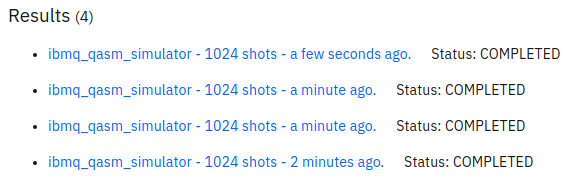
\includegraphics[width=.8\textwidth]{figures/time_expr.png} 
	\caption{Časy dokončení meraní experimetov.}
    \label{expr_time}
\end{figure}


Samozrejme, že ak potrebujeme presné merania, je lepšie použiť kompletný
simulátor. No výhodou nášho riešenia je zobrazenie zmien stavov kvantových
bitov. IBM QX dokáže zobraziť len skolabované výsledky meraní, i keď veľmi
presne, no niekedy je vhodnejšie vedieť stav ešte pred kolabovaním. Náš 
pravdepodobnosný model generuje stromovú štruktúru, v ktorej si zaznamenáva
priebežné stavy kvantových bitov. Získané stromy z našich experimentov sme 
pridali do príloh tejto práce.

Funkčnosť modelu sme otestovali na troch experimetoch. V každom experimente 
sme odvodili vzorce pre výpočet pravdepodobností kolabovania do jednotlivých
stavov pre všetky definované časové okamihy. Uviedli sme výsledky, ktoré 
sú dosiahnuteľné pomocou kvantového stroja IBM Quantum Experience. Nakoniec 
sme pre každý experiment uskutočnili meranie pomocou nášho pravdepodobnostného
modelu.

V neposlednej rade sme preskúmali aj možnosť využitia tohto pravdepodobnostného
modelu aj pri zložitejšom príklade, v ktorom prebiehal kvantový jav zvaný
kvantová teleportácia.

% !TEX root = ../thesis.tex

\chapter{Záver}
Úlohou tejto práce bolo zostaviť programové riešenie problému merania
stavov kvantových bitov počas behu kvantového obvodu. Poskytli sme výstižný
úvod do problematiky kvantových počítačov z pohľadu matematických 
definýcií. Po prečítaní tejto práce by aj laikovy malo byť jasné ako prebieha
kvantový obvod, a na akom princípe fungujú merania bitov.

Ešte pred samotnou implementáciou Haskellovského programu sme sa snažili 
detailne priblížiť na akom matematickom princípre postavíme pravdepodobnostný
model. Analýzu návrhu a proces implementácie tohto pravdepodobnostného modelu
sme rozobrali v jednej z kapitol. Vďaka tomu sme mohli ukázať aj riešenie 
zložitejšieho príkladu kvantového obvodu.

Tak ako sme dokázali pri experimentoch, náš pravdepodobnostný model je 
využiteľný pri tvorbe a analýze kvatnových obvodov. Značne urýchľuje výpočty,
ktoré je nutné vykonávať a odvodzovať pri práci s spomínanými obvodmi.
Poskytuje grafickú podobu zmien stavov, čo len ďalej zjednodušuje pochopenie
práce kvantových počítačov.

Do budúcna by bolo dobré vytvoriť grafické prostredie, ktoré by bolo 
nadstavbov tejto práce. Uľahčilo by to prácu, nakoľko by nebolo nutné poznať
jazyk Haskell pre realizáciu experimentu. Experimenty, ktoré táto práca 
popisuje sú ale dobrým návodom ako tento program využívať. Taktiež obohatenie 
tohto pravdepodobnostného modelu o sofistikovanejší simulátor kvantového stroja
by priniesol presnejšie výsledky, najmä pri obvodoch s previazanými kvantovými
bitmi. V takom prípade by bolo možné úplne nahradiť kvantový simulátor
IBM Quantum Experience, pri návrhu a prvotnom testovaní kvantových obvodoch,
čo by v konečnom dôsledku malo za vpliv rýchlejší rozvoj tejto technológie.


% good linebraking of bibtex url
\setcounter{biburllcpenalty}{7000}
\setcounter{biburlucpenalty}{8000}

%% The bibliography
\phantomsection
\addcontentsline{toc}{chapter}{Literatúra}
\printbibliography[title={Literatúra}]

% List of acronyms
\printglossary[type=\acronymtype,title={\acrlistname}]

%% Appendix
%% !TEX root = ../thesis.tex

\chapter*{Zoznam príloh}
\addcontentsline{toc}{chapter}{Zoznam príloh}

\begin{description}
	\item[Príloha A] Lorem ipsum
    \item[Príloha B] CD médium -- záverečná práca v~elektronickej podobe,
    \item[Príloha C] Používateľská príručka
    \item[Príloha D] Systémová príručka
\end{description}

%\appendix
%\renewcommand\chaptername{Príloha}
%% !TEX root = ../thesis.tex



% zivotopis autora
%\curriculumvitae\protect
%Táto časť\/ je nepovinná. Autor tu môže uviesť\/ svoje biografické
%údaje, údaje o~záujmoch, účasti na~projektoch, účasti na~súťažiach,
%získané ocenenia, zahraničné pobyty na~praxi, domácu prax, publikácie
%a~pod.

\end{document}
